\documentclass[../DS03.tex]{subfiles}%
\graphicspath{{./figures/}}%

\begin{document}%

\section[60]"P"{Décrément logarithmique électrique}
\enonce{%
	On étudie la réponse $u(t)$ à un échelon de tension $e(t)$ tel que
	$ \left\{
		\begin{array}{rcl}
			e(t<0)    & = & 0 \\
			e(t\geq0) & = & E
		\end{array}
		\right.$
	dans le circuit ci-dessous.
	\begin{center}
		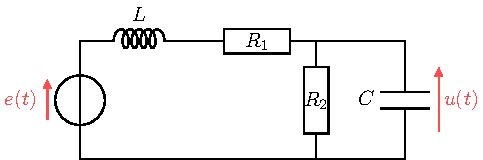
\includegraphics[width=.5\linewidth]{dec_log-plain}
	\end{center}
}%

\QR[4]{%
	Déterminer la valeur $u_{\infty}$ vers laquelle tend $u(t)$ lorsque $t
		\longrightarrow \infty$.
}{%
	$R_2$ et $C$ sont en parallèle, donc $u(t)$ est à la fois la tension aux
	bornes de $C$ et de $R_2$.
	\smallbreak
	\begin{isd}
		De plus, à $t \longrightarrow \infty$, la bobine
		se comporte comme un fil et le condensateur comme un interrupteur ouvert. Le
		circuit est donc équivalent à un diviseur de tension \pt{1} avec $R_1$ et $R_2$ en
		série alimentées par la tension $e(t)$, et on a donc
		\[ \boxed{u(\infty) \stm{=} u_{\infty} = \frac{R_2}{R_1 + R_2}E}\]
		\tcblower
		\begin{center}
			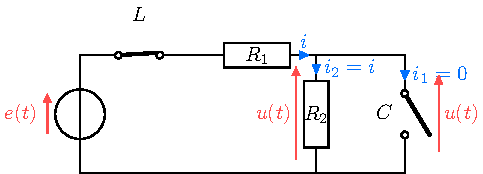
\includegraphics[width=\linewidth]{dec_log-RP}
			\captionof{figure}{Schéma équivalent. \protect\pt{1}+\protect\pt{1}}
		\end{center}
	\end{isd}
	\vspace{-15pt}
}%

\QR[8]{%
Montrer que $\DS \dv[2]{u}{t} + 2\lambda \dv{u}{t} +\w_0{}^2 u =
	\w_0{}^2u_{\infty}$. Exprimer $\lambda$ et $\w_0$ en fonction de $L$, $C$,
$R_1$ et $R_2$.
}{%
On applique les lois de \textsc{Kirchhoff}~:
\smallbreak
\begin{isd}
	Avec une loi des mailles et les relations courant-tension~:
	\[ u + L \dv{i}{t} + R_1i \stm(un){\stm{=}} E\]
	\tcblower
	Avec la loi des nœuds~:
	\begin{gather*}
		i \stm{=} i_1 + i_2 \stm{=} C \dv{u}{t} + \frac{u}{R_2}
	\end{gather*}
\end{isd}
\begin{align*}
	\beforetext{En combinant~:}
	u + L \dv{}{t} \left( C \dv{u}{t} + \frac{u}{R_2} \right) + R_1C
	\dv{u}{t} + R_1\frac{u}{R_2}                                          & = E
	\\\Lra
	u + LC \dv[2]{u}{t} + \frac{L}{R_2} \dv{u}{t} +
	R_1C \dv{u}{t} + \frac{R_1}{R_2}u                                     & = E
	\\\Lra
	LC \dv[2]{u}{t} + \left( \frac{L}{R_2} + R_1C
	\right)\dv{u}{t} + \left( \frac{R_1}{R_2} + \underset{
	\frac{R_2}{R_2}}{\cancel{1}} \right)u                                 & \stm{=} E
	\\\Lra
	\dv[2]{u}{t} + \left( \frac{1}{R_2C} + \frac{R_1}{L}
	\right) \dv{u}{t} + \left( \frac{R_1 + R_2}{R_2} \right) \frac{u}{LC} & =
	\frac{E}{LC}
	\\\Lra
	\dv[2]{u}{t} + \left( \frac{1}{R_2C} + \frac{R_1}{L}
	\right) \dv{u}{t} +\left( \frac{R_1 + R_2}{R_2} \right)
	\frac{u}{LC}                                                          & \stm{=} \left(\frac{R_1 + R_2}{R_2}\right)
	\frac{u_{\infty}}{LC}
	\\\Lra
	\Aboxed{\dv[2]{u}{t} + 2\lambda \dv{u}{t} + \w_0{}^2u                 & =
		\w_0{}^2u_\infty}
\end{align*}
\begin{gather*}
	\text{avec} \quad
	\boxed{
		\w_0 \stm{=} \sqrt{\frac{1}{LC} \left( \frac{R_1 +
				R_2}{R_2} \right)}
	}
	\qet
	\boxed{
		\lambda \stm{=} \frac{1}{2} \left(
		\frac{1}{R_2C} + \frac{R_1}{L} \right)
	}
\end{gather*}
}%

\QR[10]{%
	Exprimer la forme générale de $u(t)$ en fonction de $u_{\infty}$,
	$\lambda$, de la pulsation et de deux constantes d'intégration qu'on ne
	cherche pas à déterminer pour le moment.
}{%
	Pour la solution de l'équation homogène, on injecte $u_h(t) = K\exr^{rt}$
	\pt{1} la forme générique pour obtenir l'équation caractéristique. On en
	cherche alors les racines grâce au discriminant $\Delta$~:
	\begin{gather*}
		r^2 + 2\lambda r + \w_0{}^2 \stm{=} 0
		\Rightarrow
		\Delta \stm{=} 4(\lambda^2 - \w_0{}^2)
	\end{gather*}
	On sait que $\Delta < 0$ \pt{1} puisqu'on observe des oscillations amorties.
	On aura donc
	\begin{gather*}
		r_\pm \stm{=}
		-\frac{\cancel{2}\lambda}{\cancel{2}}
		\pm \jj \frac{1}{\bcancel{2}}\sqrt{\bcancel{4}(\w_0{}^2 - \lambda^2)}
		\Leftrightarrow
		\boxed{r_\pm \stm{=} -\lambda \pm \jj \W}
		\qavec
		\boxed{\W \stm{=} \sqrt{\w_0{}^2 - \lambda^2}}
	\end{gather*}
	La solution particulière étant visiblement $u_p = u_\infty$ \pt{1}, on aura la
	forme générale
	\begin{equation*}
		u(t) \stm{=} u_h(t) + up
		\Lra
		\boxed{%
			u(t) \stm{=} \exr^{-\lambda t} \left( A\cos\Wt + B\sin\Wt \right) + u_\infty
		}
	\end{equation*}
}%

\QR[9]{%
	Justifier entièrement les conditions initiales. Deux schémas sont attendus.
}{%
	\begin{isd}
		\tcbsubtitle{\fatbox{\textbf{En $t = 0^-$}}}
		Or, avant l'échelon montant, le générateur est éteint depuis longtemps.
		Ainsi,
		le condensateur est déchargé, et $\boxed{u(0^-) = 0}$ \pt{1}, et aucun
		courant
		ne
		circule dans le circuit, donc $\boxed{i(0^-) = 0}$ \pt{1}.
		\begin{center}
			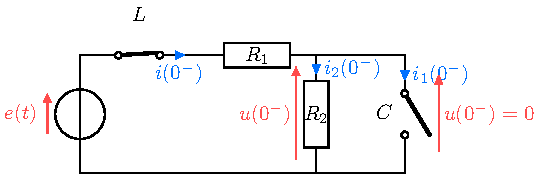
\includegraphics[width=\linewidth]{dec_log-0m}
			\captionof{figure}{Schéma en $t = 0^-$. \protect\pt{1}}
		\end{center}
		\tcblower
		\tcbsubtitle{\fatbox{\textbf{En $t = 0^+$}}}
		Or, par continuité de l'intensité traversant une bobine et de la tension aux
		bornes d'un condensateur \pt{1}, lors de l'échelon de tension on garde
		$\boxed{i(0^+)
				= i (0^-) = 0}$ et $\boxed{u(0^+) = u (0^-) = 0}$ \pt{1}.
		\begin{center}
			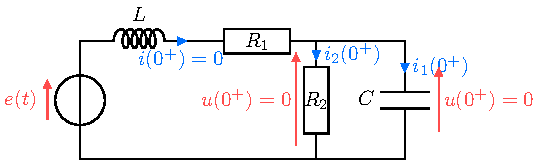
\includegraphics[width=\linewidth]{dec_log-0p}
			\captionof{figure}{Schéma en $t = 0^+$. \protect\pt{1}}
		\end{center}
	\end{isd}
	Ainsi, avec une loi des nœuds, on a $i(0^+) = i_1(0^+) + i_2(0^+)$ \pt{1}.
	Seulement, comme $i_2(0^+)$ est le courant passant dans la résistance $R_2$ de
	tension
	$u(0^+) = 0$, on a $i_2(0^+) = u(0^+)/R = 0$ \pt{1}, soit avec la loi des
	nœuds, $\boxed{i_1(0^+) = 0 \stm{=} C \eval{\dv{u}{t}}_{0^+}}$.
}%

\QR[3]{%
	Déterminer alors l'expression complète de $u(t)$ en fonction de $u_{\infty}$,
	$\lambda$ et $\W$.
}{%
	\begin{isd}[sidebyside align=top]
		\tcbsubtitle{\fatbox{\textbf{Première condition}}}
		\vspace{-15pt}
		\begin{gather*}
			u(0) = 0
			\Lra
			A + u_{\infty} = 0
			\Lra
			\boxed{A \stm{=} -u_{\infty}}
		\end{gather*}
		\tcblower
		\tcbsubtitle{\fatbox{\textbf{Seconde condition}}}
		\vspace{-15pt}
		\begin{gather*}
			\eval{\dv{u}{t}}_{0} = 0
			\Lra
			-\lambda A + B\W = 0
			\Lra
			\boxed{B \stm{=} \frac{-\lambda u_{\infty}}{\W}}
		\end{gather*}
	\end{isd}
	\begin{gather*}
		\beforetext{Finalement,}
		\boxed{u(t) \stm{=}
			u_{\infty} \left(
			1 - \exr^{-\lambda t}
			\left( \cos(\Wt) + \frac{\lambda}{\W} \sin(\Wt) \right)
			\right)
		}
	\end{gather*}
}%

\enonce{%
	\smallbreak
	\noindent
	\begin{minipage}{0.48\linewidth}
		On observe à l'oscilloscope la courbe $u(t)$ ci-contre.
	\end{minipage}
	\begin{minipage}{0.48\linewidth}
		\centering
		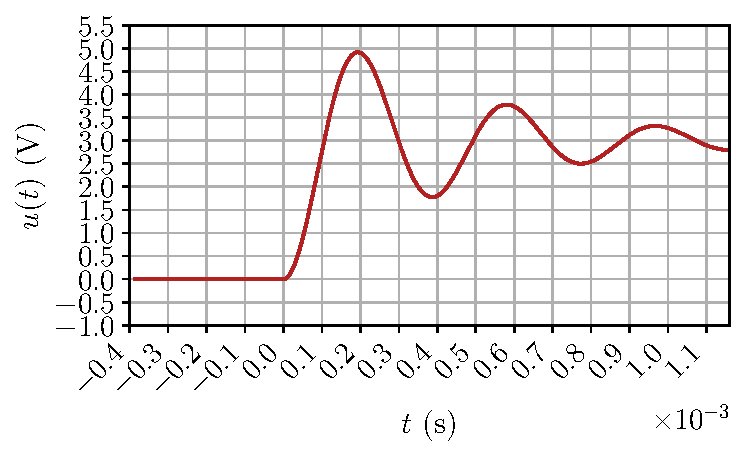
\includegraphics[width=\linewidth]{dec_log_courbe}
	\end{minipage}
}%

\QR[4]{%
	Déterminer, en détaillant vos points de mesures, la valeur numérique
	de la pseudo-période $T$.
}{%
	On lit l'abscisse du premier et du troisième maximum, qu'on appelle
	$t_1$ et $t_3$ respectivement. On a alors
	\begin{gather*}
		2T = t_3 - t_1
		\Lra
		\boxed{T \stm{=} \frac{t_3-t_1}{2}}
		\qav
		\left\{
		\begin{array}{rcl}
			t_3 & \stm{=} & \SI{0.95e-3}{s}
			\\
			t_1 & \stm{=} & \SI{0.19e-3}{s}
		\end{array}
		\right.\\
		\AN
		\xul{
			T \stm{=} \SI{3.8e-4}{s}
		}
	\end{gather*}
}%

\QR[4]{%
Déterminer, en détaillant vos points de mesures, la valeur numérique
du décrément logarithmique
\[\boxed{ \delta = \frac{1}{n} \ln \left( \frac{u(t) -
	u_{\infty}}{u(t+nT)-u_{\infty}} \right)}\]
}{%
On calcule $\delta$ avec deux pseudo-périodes ici. On lit la valeur de tension
aux premier et troisième pics, à $t_1$ et $t_3$ respectivement, ainsi que ce qui
semble être la valeur limite $u_{\infty}$~:
\begin{gather*}
	\boxed{
		\delta =
		\frac{1}{2} \ln \left( \frac{u(t_1) - u_{\infty}}{u(t_3) - u_{\infty}} \right)
	}
	\qav
	\left\{
	\begin{array}{rcl}
		u(t_1)     & \stm{=} & \SI{4.9}{V}
		\\
		u(t_3)     & \stm{=} & \SI{3.3}{V}
		\\
		u_{\infty} & \stm{=} & \SI{3.0}{V}
	\end{array}
	\right.\\
	\AN
	\xul{
		\delta \stm{=} \num{0.92}
	}
\end{gather*}
}%

\QR[5]{%
	Déterminer la relation entre $\delta$, $\lambda$ et $T$. En déduire la
	valeur numérique de $\lambda$.
}{%
	Avec l'expression de $u(t)$, on peut développer le dénominateur de
	$\delta$~:
	\begin{gather*}
		u(t+nT) - u_\infty \stm{=} \exr^{-\lambda nT}\times
		\underbracket[1pt]{\exr^{-\lambda t}
			\bigg(
			A\underset{=\cos\Wt}{\underline{\cos(\Wt+n\Wt)}} +
			B\underset{=\sin\Wt}{\underline{\sin(\Wt+n\Wt)}}\bigg)
		}_{u(t) - u_\infty \pt{1}}
		\\
		\beforetext{Ainsi,}
		\frac{u(t) - u_\infty}{u(t+nT)-u_\infty} \stm{=} \exr^{+\lambda nT}
		\Rightarrow
		\delta = \frac{1}{n} \ln (\exr^{\lambda nT})\\
		\Leftrightarrow
		\boxed{%
			\delta = \lambda T
			\Lra
			\lambda \stm{=} \frac{\delta}{T}
		}%
		\qavec
		\left\{
		\begin{array}{rcl}
			\delta & = & \num{0.92}     \\
			T      & = & \SI{3.8e-4}{s}
		\end{array}
		\right.\\
		\AN
		\xul{\lambda \stm{=} \SI{2.3e3}{s^{-1}}}
	\end{gather*}
}

\QR[2]{%
	Sachant que $R_1 = \SI{1.0}{k\ohm}$, $R_2 = \SI{50}{k\ohm}$ et $L =
		\SI{500}{mH}$, déterminer la valeur de $C$.
}{%
	On sait que $\lambda$ s'exprime en fonction de $C$, on l'isole donc de son
	expression~:
	\begin{gather*}
		2\lambda = \frac{1}{R_2C} + \frac{R_1}{L}
		\Leftrightarrow
		R_2C = \frac{1}{2\lambda - \frac{R_1}{L}}\\
		\Leftrightarrow
		\boxed{C \stm{=} \frac{1}{2R_2\lambda - \frac{R_1R_2}{L}}}
		\qavec
		\left\{
		\begin{array}{rcl}
			R_1     & = & \SI{1.0}{k\ohm}    \\
			R_2     & = & \SI{50}{k\ohm}     \\
			L       & = & \SI{500}{mH}       \\
			\lambda & = & \SI{2.3e3}{s^{-1}}
		\end{array}
		\right.\\
		\AN
		\xul{C \stm{=} \SI{7.6}{nF}}
	\end{gather*}
}

\end{document}
